\section{ViSIT Metadaten und die Semantische Datenbank}\label{sec:semantics}

Brainstorm, things to write about:

\begin{itemize}
	\item theoretischer background: rdf daten, CIDOC, Vismo
	\item datenbank: infrastruktur (hosting, allgemeiner zugriff von aussen), drupal, wisski (allgemein), grundfunktionalität
	\item wisski: rdf daten, pfade, konfiguration
	\item REST API: allgemeine beschreibung
	\item zusatzfeatures: copy and paste, excel import
\end{itemize}

\subsection{Theoretische Grundlagen für die Semantische Datenbank}\label{sec:theoreticalBackground}

Dieses Unterkapitel gibt Einblicke in Teilbereiche des Semantic Webs, um eine theoretische Grundlage für die folgenden technischen Entwicklungen zu geben. Nachdem diese erläutert wurden, wird ebenfalls auf eine spezielle Ausprägung eines Metadatenmodells eingegangen, welches die Struktur für die im ViSIT Projekt verwendeten Metadaten vorgibt: das ViSIT Model \textbf{VisMo}.

Die hier angeführten Ausführungen beschränken sich jedoch nur auf jeweilige Grundlagen der Themenkomplexe, welche an manchen Stellen um weiterführende Informationen erweitert werden, wenn dies für den weiteren Verlauf von Nöten ist. Dennoch, falls angestrebt, verweisen wir für ein tieferes Verständnis auf weitere Fachliteratur, wie z.B. \cite{Hitzler-SemanticWeb-2007}.

\paragraph{Semantic Web und RDF Daten}

Das Semantic Web ist eine Art Erweiterung zum eigentlichen World Wide Web, wie wir es aktuell kennen. Dieses ist primär für Menschen ausgelegt, die durch Homepages browsen und dabei entsprechende Informationen durch betrachten und lesen der Homepages erlangen. Diese Informationen sind dadurch jedoch nur für Menschen vorhanden, Maschinen oder Computer können auf die Informationen nicht zugreifen, um mit den entsprechenden Daten arbeiten zu können. Genau hier setzt das Semantic Web an, welches Standardisierungen, Regeln und Prozesse vorgibt, um Homepages und Applikationen so anzupassen, dass eben genau eine (semi-) automatische Informationsverarbeitung für Maschinen möglich wird.
 
Eine dieser Standardisierungen ist das Resource Description Framework \textbf{RDF} \cite{Manola-RDFPrimer1.0-2004}, welches der de-facto Standart im Semantic Web ist, um Metadaten zu beschreiben. Daten in RDF werden als Graph modelliert und persistiert, welcher aus Knoten und Kanten besteht. Dabei entsteht eine Wissensbasis gefüllt an Informationen. Die Knoten sind hierbei die \q{Akteure}, also diejenigen Entitäten, Sachen, Objekte, Dinge etc., ausgehend vom jeweiligen Anwendungsfall, auf die sich die im Graphen enthaltenen Informationen beziehen (diese Dinge werden im Folgenden weiterhin als \q{Metadatenentität} bezeichnet). Die Kanten im Graphen beschreiben Beziehungen zwischen den gegebenen Knoten und Eigenschaften der Knoten. Weiterhin sind die Knoten und Kanten durch das Grundprinzip eines \textbf{Statements} verbunden, welches eine Kapselung einer elementaren Aussage darstellt. Das Statement ist, ähnlich dem deutschen Satzbau, immer bestehend aus drei Teilen:

\begin{description}
	\item[Subjekt] Die Metadatenentität repräsentiert als ein Knoten im Graphen, von der die Aussage - und damit das Prädikat - des Statements ausgeht.
	\item[Prädikat] Die Semantik oder die Bedeutung der Aussage.
	\item[Objekt] Zweierlei Konzepte können das Objekt des Statements bilden: ein weiterer Knoten im Graphen, um das Ziel der Aussage und damit des Prädikats, um eine Relation zwischen zwei Metadatenentitäten/Knoten darzustellen, oder ein fester Wert, um eine Eigenschaft einer Metadatenentitäten/eines Knotens zu charakterisieren.
\end{description}

Zur Verständlichkeit für die Thematik der Aussagen und Statements im Semantic Web Kontext, soll hier ein kurzes, erfundenes Beispiel erläutert werden. Folgende Aussagen bilden die Wissensbasis:

\begin{itemize}
	\item Peter ist vom Beruf Baumeister.
	\item Peter ist 40 Jahre alt.
	\item Peter war am Bau des Steinschlosses beteiligt.
	\item Das Steinschloss besteht aus Stein.
	\item Das Steinschloss ist 10 Jahre alt.
\end{itemize}

Wie oben beschrieben, bestehen die Aussagen jeweils aus Subjekt, Prädikat und Objekt. Als Subjekte agieren die beiden Metadatenentitäten \q{Peter} und das \q{Steinschloss}, während die Objekte der Aussagen der Beruf \q{Baumeister}, das Material \q{Stein}, zwei \q{Altersangaben}, sowie das \q{Steinschloss} selbst sind. Semantisch sind die Subjekte und Objekte über die Beziehungen bzw. Eigenschaften einer \q{Berufszuordnung}, zwei \q{Alterszuordnungen}, einer \q{Materialzuweisung} sowie der \q{Erbauung} eines Objekts verbunden.

Diese Aussagen können nun in einen Graphen zusammengefasst werden, dessen high-level Illustration in \autoref{fig:statements} zu sehen ist.

\begin{figure}[htb]
    \centering
    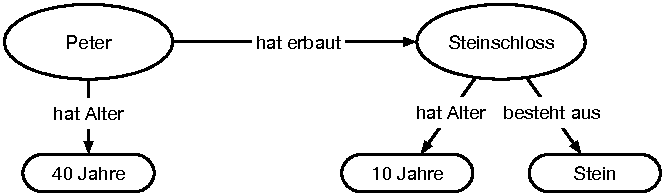
\includegraphics[width=\textwidth]{Figures/berndl/statements}
    \caption{\label{fig:statements} Informationen aus obigen Aussagen, kombiniert als Graph.}
\end{figure}

\paragraph{Linked Open Data Gedanke}

Ein weiterer Eckpfeiler des Semantic Web ist ein weiteres Konzept, das unter dem Namen \textbf{Linked Open Data - LOD} bekannt ist. Oft wird dieser Name ebenfalls für das Semantic Web selbst benutzt, die punktgenauen Definitionen überschneiden und ergänzen sich.

Einfach übersetzt zielt LOD auf öffentlich zugängliche Daten ab, die untereinander vernetzt und verlinkt sind. Somit soll es möglich sein, verteilte Datenbanken mit ihren eigenen entsprechenden Wissensbasen, miteinander zu verbinden, um so jedem Beteiligten mehr Informationen zur Verfügung zu stellen, da durch die Verlinkung einzelner Graphen ein großer Gesamtgraph entsteht. Auf diese Weise macht es Sinn, dass jede Wissensbasis ihren eigenen spezialisierten Kontext besitzt. Sollte eine Wissensbasis weitere Informationen aus einem anderen Kontext benötigen, müssen diese Daten nicht auf eigene Hand erforscht und aufbereitet werden, da eine LOD Verbindung zu einer anderen Wissensbasis hergestellt werden kann. Zur weiteren Veranschaulichung dieser Thematik und dessen Vorteile, zeigt der folgende Paragraph zwei Anwendungsfälle im geschichtswissenschaftlichen Kontext.

\paragraph{Zwei Anwendungsfälle für RDF im Geschichtswissenschaftlichen Kontext}

Ein erster Anwendungsfall, von dem geisteswissenschaftliche Wissensbasen profitieren können, ist oben bereits kurz angedeutet worden: das Verbinden einer eigenen Wissensbasis mit externen, bereits bestehenden Wissensbasen. Das Erforschen und Erkunden von Wissen benötigt generell in jeglichem Kontext sehr viel Zeit und ebenfalls Pflege der Daten. Daher kommt diesem Anwendungsfall der LOD Gedanke entgegen, da bereits erstellte Wissensbasen und deren Datenbanken öffentlich zugänglich sind.

Gerade generelle Themen oder Kontexte wie Personen, Städte oder Orte werden in vielen geschichtswissenschaftlichen Projekten benötigt, und gerade diese sind in öffentlichen Datenbanken zugänglich. Daher ist es für diese Anwendungsfälle sinnvoll, den eigens entwickelten Anwendungsfall an diese Datenbanken zu knüpfen. Dadurch wird der eigene Zeitaufwand erheblich reduziert und die angebundenen Daten genießen in der Regel außerdem einen hohen Standard, da bereits viele potenzielle Reviews von anderen Nutzern bestehen.

Ein zweiter großer Vorteil davon, geschichtswissenschaftliche Daten in Form von Metadaten und RDF zu persistieren, ist das mögliche Erschließen von vorher nicht bekannten oder erforschten Zusammenhänge der persistierten Objekte. Dazu folgendes (frei erfundenes) Beispiel: Ausgehend von der eigenen Wissensbasis, die die Daten aus \autoref{fig:statements} enthält, sollen nun zwei weitere Wissensbasen angekoppelt werden, welche auf der einen Seite weitere Informationen über Personen und vor allem deren familiärer Beziehungen beinhaltet, und auf der anderen Seite eine Wissensbasis, die mehr Informationen über Gebäude und deren Geschichte beinhaltet. Dies ist in \autoref{fig:extendedStatements} visualisiert.

\begin{figure}[htb]
    \centering
    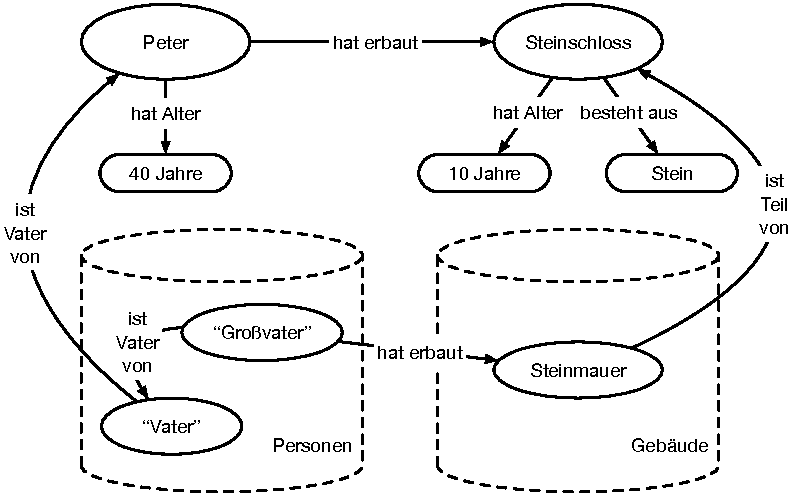
\includegraphics[width=\textwidth]{Figures/berndl/extendedStatements}
    \caption{\label{fig:extendedStatements} Grundlegende eigene Wissensbasis (oben), erweitert um zwei externe Wissensbasen (unten).}
\end{figure}

In dem Beispiel beinhaltet die eigene Wissensbasis Informationen über \q{Peter} und das \q{Steinschloss}. Durch die beiden hinzugenommenen Wissensbasen wird Peter aus dem Anwendungsbeispiel mit seinem \q{Vater}, und dieser wiederum mit seinem \q{Großvater} verbunden (die Namen sind hier zur Einfachheit ersetzt). Zudem wird die \q{Steinmauer} als ein Teil des Steinschlosses deklariert. Die beiden neuen Wissensbasen enthalten darüber hinaus bereits implizit eine eigene Verbindung, die semantisch besagt, dass der \q{Großvater} am Bau der Steinmauer beteiligt ist.

Dadurch erweitern die beiden externen Wissensbasen die eigenen Informationen durch die neu erstellten Relationen. Darüber hinaus jedoch lässt sich so ebenfalls eine neue Erkenntnis in den Daten schliessen: sowohl \q{Peter} als auch dessen \q{Großvater} sind direkt oder indirekt am Bau des \q{Steinschlosses} beteiligt.

\paragraph{Das Contextual Reference Model - CIDOC CRM}

Bisher war die technische Beschreibung der semantischen Daten im ViSIT Kontext aus Gründen der Einfachheit sehr flach gehalten. Gemäß den Semantic Web Standards basieren die Metadaten jedoch auf einem Datenmodell, um die Anforderungen des Semantic Webs zu genügen und ebenfalls technische Verabeitbarkeit zu gewährleisten.

In ViSIT ist die Wahl hierbei auf das \textbf{Contextual Reference Model CIDOC CRM} \cite{CIDOC-Doerr-2003} gefallen, da dies eine der bekanntesten und vorherrschendsten Ontologien im Bereich des kulturellen Erbes ist. Diese Ontologie wird als Basis benutzt, die im folgenden Paragraphen erweitert für den ViSIT Kontext beschrieben wird. Der größte Vorteil dieser Ontologie ist, dass sie sich nicht auf einen speziellen Bereich des kulturellem Erbes fokussiert ist, sondern auf generische Weise komplexe Zusammenhänge und verschiedene Themengebiete abbildet. Zudem solle es möglich sein, andere Ontologien oder Modelle aus dem selben Bereich in diese Ontologie zu überführen, um eine gemeinsam verständliche Wissensbasis zu kreieren.

Das CIDOC CRM wird seit mittlerweile über 10 Jahren von der CIDOC Documentation Standards Working Group\footnote{\url{http://network.icom.museum/cidoc/working-groups/overview/}} und der CIDOC CRM SIG\footnote{\url{http://network.icom.museum/cidoc/working-groups/crm-special-interest-group/}} entwickelt, welche beide Arbeitsgruppen von CIDOC\footnote{\url{http://network.icom.museum/cidoc/}} sind. Das CIDOC CRM ist 2000 als \q{Working Draft} bei der ISO/TC46/SC4\footnote{\url{https://www.iso.org/committee/48798.html}} akzeptiert worden, welcher 2006 schliesslich auch als offizieller Standard \cite{CIDOCCRM-iso21127:2006} akzeptiert wurde, und 2014 in eine überarbeitete Version \cite{CIDOCCRM-iso21127:2014} überführt wurde.

In der aktuellen Hauptversion 6.2\footnote{\url{http://www.cidoc-crm.org/Version/version-6.2}}, die im Mai 2015 veröffentlicht wurde, enthält die Ontologie 89 RDF Klassen und 149 einzigartige Relationen und Eigenschaften, die sich in einer mehrfach ineinander- sowie auseinander verzweigenden Struktur einordnen. Laufend werden ebenfalls Nebenversionen veröffentlicht - die aktuellste Versionsnummer lautet 6.2.3\footnote{\url{http://www.cidoc-crm.org/Version/version-6.2.3}}.

\paragraph{Das ViSIT Model - VisMo}

Aufbauend auf dem CIDOC CRM wurde eine Ontologie entwickelt, die den kompletten Anwendungsfall des ViSIT Projekt abbilden kann: das \textbf{ViSIT Model VisMo}. Der Fokus liegt dabei auf der Darstellung von Architektur-Objekten und Ausstellungsobjekten, die mit Personen oder Gruppen von Personen, Orten sowie zeitlichen Events in Verbindung gesetzt werden, um eine Wissensbasis zu kreieren.

Diesbezüglich sind die Hauptentitäten, die in der \visit Datenbank angelegt werden können, die folgenden:

\begin{description}
	\item[Ereignis (Activity):] Diese Entität umfasst alle vergangenen und zukünftigen Vorgänge und Geschehnisse in kulturellen, sozialen und physischen Systemen, analog zum \texttt{\q{E5\_Event}}\footnote{\url{http://www.cidoc-crm.org/Entity/E5-Event/Version-6.2}} des CIDOC CRM.
	\item[Bauwerk (Architecture):] Diese Entität bezeichnet alle Arten von Bauten, die wie die Objekte als Informationsträger (vgl. \texttt{\q{E84\_\-In\-for\-ma\-tion\_Car\-rier}}\footnote{\url{http://www.cidoc-crm.org/Entity/E84-Information-Carrier/Version-6.2}} des CIDOC CRM) betrachtet werden.
	\item[Gruppe (Group):] Diese Entität bezeichnet mehrere Personen, die sich zu einer Gruppierung zusammengeschlossen haben und durch eine gleiche oder ähnliche Tätigkeit miteinander verbunden sind (vgl. \texttt{\q{E74\_\-Group}}\footnote{\url{http://www.cidoc-crm.org/Entity/E74-Group/Version-6.2}} des CIDOC CRM).
	\item[Institution (Institution):] Diese Entität bezeichnet hier alle Arten von organisierten Einrichtungen, die keine natürlichen Personen oder Personengruppen sind, z.B. Museen, Archive, Bibliotheken, Universitäten usw.
	\item[Objekt (Object):] Diese Entität bezeichnet alle Arten von Ausstellungsobjekten aus den Sammlungen von musealen oder museumsähnlichen Institutionen, Archiven etc. , die wie Bauwerke als Informationsträger betrachtet werden (vgl. \texttt{\q{E84\_\-In\-for\-ma\-tion\_Car\-rier}}\footnote{\url{http://www.cidoc-crm.org/Entity/E84-Information-Carrier/Version-6.2}} des CIDOC CRM).
	\item[Person (Person):] Diese Entität bezeichnet analog zur Definition im CIDOC CRM der \texttt{\q{E21\_Person}}\footnote{\url{http://www.cidoc-crm.org/Entity/E21-Person/Version-6.2)}} alle natürlichen Personen, die leben oder bereits verstorben sind sowie Personen, von denen angenommen wird, dass sie lebten. Dazu zählen historische Persönlichkeiten als auch Personen aus Legenden, Mythen und Sagen.
	\item[Ort (Place):] Diese Entität bezeichnet hier ausschließlich über Koordinaten lokalisierbare verschwundene und bestehende Dörfer und Städte.
	\item[Literatur (Reference):] Diese Entität bezeichnet alle Arten von niedergeschriebenen und veröffentlichen Texten.
\end{description}

Dabei erfüllt VisMo genau den Zweck, den sich das CIDOC CRM als Ziel gesetzt hat: als eine semantische \q{Erweiterung} des CIDOC CRM ist der Inhalt, der für VisMo produziert wird, direkt zum größten Teil verständlich und Leser oder Benutzer des Modells können dies intuitiver, auf der Basis der Beschreibungen des CIDOC CRM, verstehen, lesen und benutzen. Dies ist dadurch begründet, dass alle Klassen und viele der Relationen und Eigenschaften durch Vererbung speziellere Konzepte der CIDOC CRM Klassen und Relationen/Eigenschaften sind. Nur einzelne Teile des VisMo sind speziell für die Ontologie hinzugefügt worden, immer wenn kein Konzept aus dem CIDOC CRM passend für eine Vererbung war. \autoref{fig:modelworkflow} visualisiert den Entwicklungsprozess hinter VisMo.

\begin{figure}[htb]
    \centering
    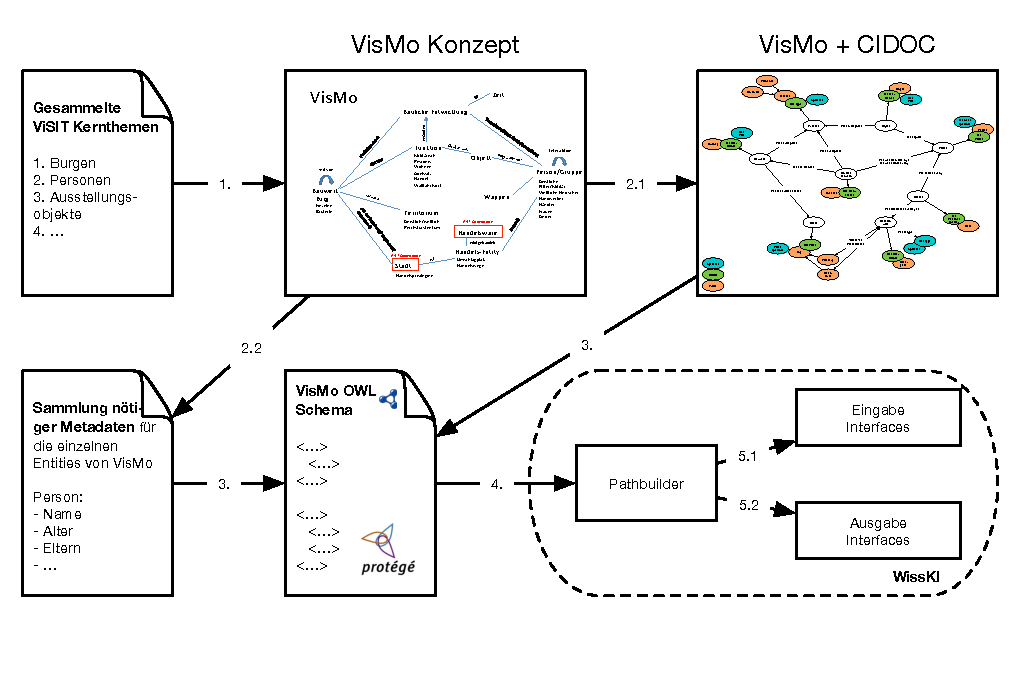
\includegraphics[width=\textwidth]{Figures/berndl/modelworkflow}
    \caption{\label{fig:modelworkflow} Arbeitsprozess hinter der Entwicklung des ViSIT Modells.}
\end{figure}

Der erste Schritt bestand dabei in der Sammlung der Kernthemen, die in ViSIT behandelt werden. Aus diesen konnte dann im nächsten Schritt ein grobes Konzept entwickelt werden, welches anschließend in RDF übertragen werden konnte. Wie oben beschrieben, wurde hierbei von CIDOC CRM Grundklassen und Relationen bzw. Eigenschaften ausgegangen, welche dann für den ViSIT Kontext erweitert und angepasst wurden. Als nächstes konnten dann die erstmals groben Konzepte und Entitäten mit benötigten Metadaten bzw. dessen Anforderungen erweitert werden. Die Ergebnisse der vorherigen Schritte konnten dann letztendlich in dem Ontologie-Editor \textbf{protegé}\footnote{\url{https://protege.stanford.edu/}} zusammengeführt werden, um eine RDF/OWL Ontologie zu erstellen. Diese ist in ihrer letzten offiziellen Version in \autoref{lst:vismo} im Appendix zu sehen.

Ebenfalls ist in \autoref{fig:modelworkflow} visualisiert, wie und an welcher Stelle die VisMo Ontologie technisch zum Einsatz kommt: sie dient als Input für das sogenannte \wisski Modul, um aus der Ontologie Ein- sowie Ausgabemasken zu generieren, welche letztendlich vom Endnutzer des ViSIT Systems benutzt werden, um einerseits Daten in die semantische Datenbank einzutragen und diese dann auch wieder auszulesen und anzuzeigen. Der große Vorteil an diesem Prozess ist, dass der Endnutzer keinerlei Wissen über das Semantic Web und seine Technologien benötigt, da der oben beschriebene Prozess davon abstrahiert. Damit schreiben und lesen die Endnutzer im Endeffekt RDF, ohne davon zu wissen. Technische Details zu diesem Prozess sowie \wisski werden in folgenden Unterkapiteln gegeben.

\subsection{Technische Details zur Semantischen Datenbank}\label{sec:technicalBackground}

Nachdem \autoref{sec:theoreticalBackground} die theoretische Grundlage für die Semantische Datenbank beschrieben hat, fokussiert sich dieses Unterkapitel auf die technischen Aspekte der Datenbank. Dazu zählt in erster Linie die \textbf{allgemeine Infrastruktur}, das \textbf{Hosting} an der Universität Passau, der \textbf{allgemeine Zugriff auf die Datenbank}, getroffene Entscheidungen bezüglich \textbf{Security und Zertifizierungen}, sowie die anschließende Beschreibung einzelner Komponenten: dem \textbf{CMS Drupal}, dessen Modul \textbf{\wisski}, die \textbf{ViSIT REST API}, der unterliegende RDF Triplestore \textbf{RDF4J} und dessen generelle Funktionalität.

Für die semantische Datenbank wurde zur Projektlaufzeit aus Testzwecken ebenfalls eine Testinstanz ins Leben gerufen, welche eine komplette Spiegelung des damals aktuellen Systems ist. Die beiden Haupt-URLs der Server sind:

\begin{itemize}
	\item \texttt{https://database.visit.uni-passau.de/}
	\item \texttt{https://database-test.visit.uni-passau.de/}
\end{itemize}

Von diesen beiden Base-URLs ausgehend sind die weiteren Komponenten über folgende URL-Zusätze zu erreichen:

\begin{itemize}
	\item \textbf{Drupal/\wisski:} Base URL + \texttt{/drupal}
	\item \textbf{RDF4J:} Base URL + \texttt{/rdf4j-workbench}
	\item \textbf{Tomcat:} Base URL (ohne Zusatz)
	\item \textbf{ViSIT REST API:} Base URL + \texttt{/metadb-rest-api}
	\item \textbf{API Beschreibung:} Base URL + \texttt{/metadb-test-api/swagger-ui.html}
\end{itemize}

\paragraph{Infrastruktur}

Die Semantische Datenbank des ViSIT Projekts ist auf einem virtuellen Server an der Universität Passau installiert. Die allgemeine Infrastruktur ist in \autoref{fig:infrastructure} zu sehen.

\begin{figure}[htb]
    \centering
    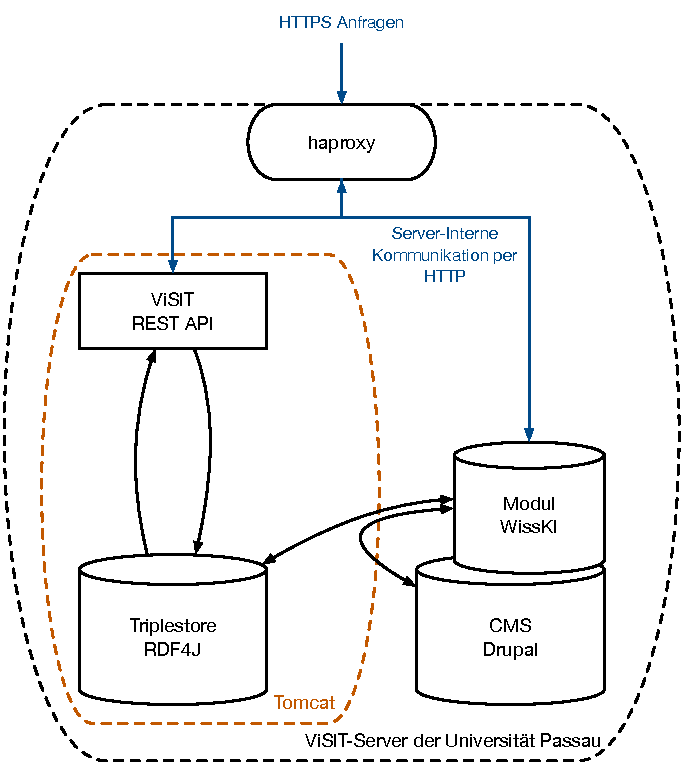
\includegraphics[width=\textwidth]{Figures/berndl/infrastructure}
    \caption{\label{fig:infrastructure} Technische Infrastruktur der Semantischen Datenbank des ViSIT Projekts.}
\end{figure}

Dessen Hauptkomponenten mit Beschreibung oder Verweis auf das ausführliche Unterkapitel sind die folgenden:

\begin{description}
	\item[haproxy] Dem virtuellen Server für die ViSIT Infrastruktur ist ein \textbf{haproxy}\footnote{\url{http://www.haproxy.org/}} vorgeschaltet. Dieser ist dafür da, die per HTTPS verschlüsselten Anfragen von aussen an den Server entgegen zu nehmen, und intern an die richtigen Komponenten weiterzuleiten. Prinzipiell kann dieser haproxy ebenfalls Anfragen per HTTP entgegen nehmen, leitet diese dann aber automatisch auf den Port für HTTPS weiter. Damit ist sicher gestellt, dass nach aussen nur verschlüsselte Daten versandt werden. Dem haproxy sind für die benötigte Funktionalität zwei backends bekannt: eines für den Tomcat (ViSIT REST API und Triplestore RDF4J) und eines für Drupal bzw. \wisski (welche hintergründig auf einem Apache laufen). Die Verschlüsselung ist durch ein SSL Zertifikat der Universität gewährleistet. Die Konfiguration zum haproxy is am Server zu finden unter \texttt{/etc/haproxy}.
	\item[Tomcat] Zur Installation weiterer Komponenten am Server, ist ein \textbf{Apache Tomcat}\footnote{\url{http://tomcat.apache.org/}} in der Version 8.5.24 installiert. Am Server ist dieser zu finden unter \texttt{/opt/tomcat8/apache-tomcat-8.5.24}.
	\item[ViSIT REST API] Diese API wurde eigens für ViSIT entwickelt, um eine Abstraktionsschicht für die unterliegenden Metadaten zu bieten. Während \wisski diese Abstraktion für die wissenschaftlichen Benutzer der Metadaten bildet, ist die API für die technische Anbindung der restlichen Komponenten des ViSIT Projekts zuständig. Die API bietet in erster Linie die Möglichkeit, die RDF Metadaten aus dem Triplestore zu lesen. Zurückgegeben wird das Ergebnis im JSON Format, um eine möglichst breite Verständnis und damit direkte Verwendbarkeit zu gewährleisten. Der zweite große Teil behandelt das Schreiben, Auslesen und Updaten der sogenannten technischen Metadaten: Metadaten, die Informationen zu einem Medien-Objekt im ViSIT Kontext geben. Die REST API ist als eigenständiges Java-Projekt implementiert, welches auf dem ViSIT Server bzw. in dessen Tomcat Installation deployed wird. Eine ausführliche Beschreibung wird in \autoref{sec:rest} gegeben.
	\item[Triplestore RDF4J] Der Triplestore ist für die Persistierung der RDF Daten zuständig. Im ViSIT Kontext ist die Wahl hierfür auf die \textbf{RDF4J}\footnote{\url{http://rdf4j.org/}} Datenbank gefallen, dieser ist jedoch durch jeglichen gleichwertigen Triplestore ersetzbar. Wie bei der REST API beschrieben, wird im ViSIT Kontext weitestgehend möglich von den RDF Daten abstrahiert. Dies wird sowohl durch die REST API und dem \wisski Modul bewerkstelligt. Der RDF4J Triplestore ist am Server bzw. in dessen Tomcat Installation deployed.
	\item[Drupal und \wisski] Die letzte Komponente der Infrastruktur der Semantischen Datenbank ist eine Kombination aus dem Content Management System \textbf{Drupal}\footnote{\url{https://www.drupal.org/}} und dessen Modul \textbf{\wisski - Wissenschaftliche KommunikationsInfrastruktur}\footnote{\url{http://wiss-ki.eu/}}. Als Modul baut \wisski auf der Implementierung von Drupal auf und benutzt dessen Funktionalität zum Persistieren von Entities als Inhalt. Zudem, da \wisski aber ebenfalls mit RDF Daten arbeitet, wird ein Triplestore benötigt - wie oben beschrieben. \wisski übernimmt dabei die Synchronisation zwischen den Entities in Drupal und den RDF Daten, sowohl beim Speichern als auch beim Auslesen von Daten. Weiterhin bietet \wisski die Möglichkeit, ein eigenes Datenmodell zu definieren, welches den gesamten Datenfluss eine Struktur vorgibt. Aus diesem werden ebenfalls einfache Interfaces generiert, um auf der einen Seite die Daten anzulegen, und auf der anderen Seite auf eine einfache Weise darzustellen. Weitere Details hierzu werden in \autoref{sec:wisski} beschrieben.
\end{description}

Im Zusammenspiel der obig genannten Komponenten erlaubt das gesamte System der Semantischen Datenbank das Management der semantischen Daten, die für den Kontext des ViSIT Projekts benötigt werden. Der Workflow der Datenbank sieht dabei in etwa wie folgt aus:

\begin{itemize}
	\item Über die einfachen \wisski Eingabe-Interfaces geben die Kuratoren bzw. Geisteswissenschaftler Informationen und Metadaten in das Gesamtsystem ein.
	\item Diese Metadaten werden mit der \wisski Funktionalität automatisch ebenfalls in RDF Daten übersetzt, die dem Schema entsprechen, welches bei Installation und Konfiguration des Gesamtsystems erstellt wird (siehe \autoref{sec:theoreticalBackground} für das Metadatenmodell CIDOC + VisMo, \autoref{sec:wisski} für die Konfiguration von \wisski).
	\item Für Forschungszwecke können diese angelegten Metadaten dann mit den \wisski Ausgabe-Interfaces betrachtet werden, was ebenfalls die Graphstrukturen hinter den Daten hervorhebt, da in den Interfaces zwischen den einzelnen Entitäten navigiert werden kann.
	\item Die ViSIT REST API dient zur technischen Anbindung weiterer ViSIT Komponenten, indem die Metadaten auf standardisierte Weise abgefragt werden können.
\end{itemize}

\subsection{\wisski - Wissenschaftliche KommunikationsInfrastruktur}\label{sec:wisski}

Das \wisski Modul bietet die Möglichkeiten, sowohl RDF Daten zu lesen und zu schreiben - aber auf eine einfache Weise über simpel gehaltene Eingabe- und Ausgabeinterfaces, um den Zugang für Forscher und die Geisteswissenschaftler im \visit Kontext zu gewährleisten. Um dies jedoch zu bewerkstelligen, benötigt das Modul verschiedene Konfigurationen und Einstellungen. Unter anderem das wichtigste ist das Definieren der semantischen Struktur der Daten, wie es bereits oben beschrieben wurde.

Für den \visit Anwendungsfall ist das technische System der semantischen Datenbank, beschrieben in \autoref{sec:semantics}, vollständig konfiguriert und betriebsbereit. Nichtsdestotrotz werden in den folgenden Unterabschnitten die Einstellungen für \wisski erläutert, um für potenziell zukünftige Änderungen eine grundlegende Beschreibung zu geben. Diese Beschreibungen können jedoch nie eine Tiefe und Genauigkeit erreichen, wie sie von den \wisski Entwicklern gegeben werden kann. Deswegen sei hier ebenfalls auf \url{http://wiss-ki.eu/} verwiesen.

\paragraph{\wisski Salz Adapter}

Wie ebenfalls bereits in \autoref{sec:technicalBackground} beschrieben, regelt das \wisski System das Persistieren und Auslesen der im Gesamtsystem angewandten semantischen Daten. Als ein Modul für das CMS Drupal, werden die Daten auf der einen Seite im CMS als Entitäten gespeichert, auf der anderen Seite - da die Daten auf Semantic Web Standards basieren sollen - als RDF Daten in einem Triplestore. \wisski führt hier automatisch die Konvertierung zwischen den beiden Datenbanken durch, ohne dass der Nutzer hier aktiv werden müsste.

Die Verbindung mit dem Drupal CMS geschieht automatisch mit der Installation des \wisski Moduls. Was jedoch konfiguriert werden muss ist die Verbindung des Moduls zum zu verwendenden Triplestore. Dies passiert im sogenannten \textbf{\wisski Salz Adapter}.  

Wenn das Menü zum bearbeiten der Adapter geöffnet wird, erscheint eine Liste der aktuell definierten Adapter. Für das \visit Projekt ist bereits ein Adapter eingerichtet mit dem Namen \texttt{visittestrepo}. Grundsätzlich reicht für einen Anwendungsfall wie \visit ein Adapter, es können aber natürlich beliebig viele Adapter definiert werden. \autoref{fig:adapter1} und \autoref{fig:adapter2} im Appendix zeigen die Konfigurationsmöglichkeiten eines \wisski Salz Adapters, bzw. die Einstellungen die für \visit getätigt wurden.

Die wichtigsten Endpunkte bzw. Konfigurationsmöglichkeiten sind die folgenden (die hier nicht erwähnten Punkte können in der Regel auf der Standardkonfiguration bzw. leer gelassen werden):

\begin{description}
	\item[Adapter Name:] Der Name des Adapters, mit dem dieser eindeutig identifiziert werden kann.
	\item[Writeable und Preferred Local Store:] Diese beiden Checkboxen sollten in der Regel immer gesetzt sein, wenn es sich um den Adapter bzw. Triplestore handelt, der hauptsächlich mit dem System arbeiten soll. \q{Writeable} bedeutet, dass Daten auf dem Triplestore geschrieben werden dürfen, \q{Preferred Local Store} weißt das System an, diesen entsprechenden Adapter als Hauptadapter zu benutzen, falls mehrere definiert sein sollten.
	\item[Read und Write URL:] Dies sind die beiden Einstellungen, die \wisski mit dem Triplestore verbinden. Es sind die beiden URLs des entsprechenden Triplestore, auf die bei diesem lesend bzw. schreibend zugegriffen werden kann. Nur wenn diese beide gesetzt sind, kann das System richtig in Betrieb genommen werden. Die beiden URLs, die in den Bildern gesetzt sind, zeigen also auf den Triplestore, der in der Infrastruktur für die semantische Datenbank installiert wurde. (Zusätzliche Hintergrundinformation: die URLs zeigen hier auf \q{\texttt{http://lo\-cal\-host:\-8081/...}} und damit auf eine lokale Installation, da sowohl das \wisski/CMS System und der Triplestore auf dem selben Server installiert ist. Die beiden Komponenten kommunizieren lokal miteinander.)
	\item[Default Graph URI:] Für RDF Daten werden eindeutige URI Bezeichner für die Knoten und Kanten des RDF Graphen benötigt. In der Regel erhalten die Knoten, wenn sie für Instanzen bzw. Entitäten stehen, eine zufällig generierte Zeichenkette als URI. Die Default Graph URI wird dann verwendet, um vor diese Zeichenkette gesetzt zu werden. Somit entstehen URI Bezeichner, die auf die Semantic Web Standards passen und auch den eigenen Anwendungsfall besser repräsentieren: so wie im Beispiel für das \visit Projekt mit \q{\texttt{http://visit.de/data}}. Eine beispielhafte URI wäre also \q{\texttt{http://visit.de/data/5c62c9aab4666}}.
	\item[Reiter Compute Type and Property Hierarchy:] Ein weiterer wichtiger Punkt im Bezug auf das Modell und damit die Struktur der semantischen Daten befindet sich im Reiter mit dem Namen \q{\texttt{Compute Type and Property Hierarchy and Domains and Ranges}}. Öffnet man den Reiter, erhält man die Möglichkeit (nachdem die Checkbox \q{\texttt{Re-Compute results}} betätigt wurde), durch den Button \q{\texttt{Start Reasoning}} einen sogenannten Reasoning Prozess zu starten. Einfach formuliert  betrachtet dieser die aktuell definierten Modelle des Systems, um potenziell zusätzliche Informationen hinzuzufügen. Dadurch kann das System auf schnellere Weise arbeiten, da diese Informationen nicht erst im produktiv laufenden Zustand des Systems hinzugefügt werden müssen. Diesen Prozess zu starten ist sehr wichtig, wenn ein \textbf{Update oder eine Änderung des Metadatenmodells passiert ist}. Der Prozess kann einige Minuten in Anspruch nehmen, bis er vollständig durchgeführt wurde.
\end{description}

\paragraph{\wisski Ontology}

In diesem Teil der Konfiguration kann die unterliegende Ontologie bzw. das Metadatenmodell für das System definiert werden. Dazu wird zunächst in einem Drop-Down Menu der Adapter ausgewählt, für den dies getan werden soll. Weiterhin muss dann eine RDFS oder OWL Schema Datei in das \wisski System hochgeladen werden. Dazu ist ein entsprechender Button vorgesehen.

Wenn bereits eine Ontologie für einen Adapter existiert, wird diese bzw. vielmehr dessen enthaltene Namensräume angezeigt. Zusätzlich gibt es dann die Möglichkeit, die aktuelle Ontologie zu löschen, womit wieder zum ursprünglichen Zustand - einer nicht vorhandenen Ontologie samt Upload Button - zurückgekehrt wird.

Auf diese Weise kann eine Ontologie ausgetauscht werden. Vorsicht jedoch hier: Beim Austauschen einer Ontologie sollte darauf geachtet werden, dass die alte Ontologie in der neuen Ontologie enthalten ist, damit die aktuell definierten Pfade (siehe nächsten Unterabschnitt) nicht invalidiert werden.

Ein Beispiel für das VisMo Modell, welches für das \visit Projekt im entsprechenden \wisski Modul definiert ist, ist in \autoref{fig:wisskiontology} im Appendix zu sehen.

\paragraph{Pathbuilders}

Die Pfade des \wisski Moduls bilden das eigentliche Herzstück, da ausgehend von diesen Pfaden alle weiteren Komponenten, wie zum Beispiel die Eingabe- sowie Ausgabeinterfaces, generiert werden. Dieser Unterabschnitt wird einen Einblick in die Konfiguration des \visit Projekts geben. Wie eingangs zu diesem Kapitel jedoch bereits erwähnt, kann dieser Einblick nie alle Details des Moduls abdecken. Deswegen sei hier nochmals auf \url{http://wiss-ki.eu/} für detailliertere und ausführlichere Erklärungen verwiesen.

Die erste Übersicht beim Navigieren auf das Pathbuilders Menü listet alle vorhandenen Pathbuilder auf, die aktuell im entsprechenden \wisski System definiert sind. Genauso wie für die Salz Adapter und die Ontologie genügt es aber auch hier, einen Pathbuilder zu benutzen. Der für das \visit Projekt konfigurierte Pathbuilder trägt den Namen \texttt{\q{visittestrepo\_pathes}}.

Wird dieser editiert, gelangt man in die Übersicht aller in diesem Pathbuilder befindlichen Pfade. Dies ist beispielhaft in \autoref{fig:pathbuilder} zu sehen.

Ein \wisski Pfad kann intern eine Gruppe (zur Gruppierung mehrerer Pfade für das selbe Objekt) oder ein wirklicher Pfad sein und besteht prinzipiell aus drei wichtigen Komponenten:

\begin{description}
	\item[ID] Eindeutiger Identifikator für den gesamten Pfad innerhalb des \wisski Sytems.
	\item[Pfad] Einzelner Knoten für eine Gruppe, oder eine Folge von RDF Knoten, Relationen und Eigenschaften, die den Pfad im RDF Graphen widerspiegeln sollen.
	\item[Datentyp] Definition des Werts des jeweiligen Pfades. Bei primitiven Datentypen endet der Pfad in einer RDF Eigenschaft, während eine sogenannte \texttt{\q{entity reference}} eine Relation, also einer Verbindung zu einem weiteren Knoten bzw. einer \wisski Entität entspricht.
\end{description}

Drei Beispiele sollen diesen Sachverhalt weiter erklären. \autoref{fig:paths1} zeigt zwei Pfade, wie sie für das \visit Projekt definiert wurden: der obere \q{Pfad} ist eine Gruppe für das allgemeine Museumsobjekt. Dessen ID ist \texttt{\q{Object}}, während der Pfad nur auf \texttt{\q{http://\-visit.\-de/\-ont\-o\-lo\-gies/\-vis\-mo/\-Ob\-ject}} gesetzt ist. Dies lässt sich dadurch erklären, dass die Gruppe für den Ursprungsknoten eines dieser Entitäten steht, welcher den RDF Typen \texttt{\q{http://\-visit.\-de/\-ont\-o\-lo\-gies/\-vis\-mo/\-Ob\-ject}} besitzen soll. Weiterhin benötigt eine Gruppe keinen Datentypen.

\begin{figure}[htb]
    \centering
    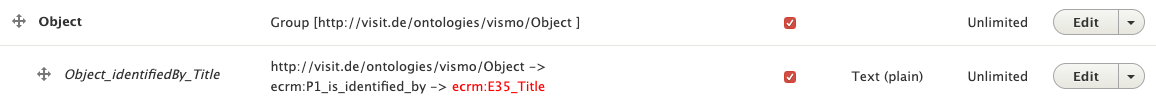
\includegraphics[width=\textwidth]{Figures/berndl/paths1}
    \caption{\label{fig:paths1} Zwei Beispiel-Pfade aus der \wisski Konfiguration des \visit Projekts.}
\end{figure}

Der zweite Pfade in \autoref{fig:paths1} ist nun ein wirklicher Pfad und steht high-level für den bezeichnenden Titel eines Ausstellungsobjekts. Die ID des Pfads ist \texttt{\q{Object\_identifiedBy\_Title}}, während der Pfad aus zwei Knoten und einer Relation besteht:

\begin{itemize}
	\item Da sich der Pfad bzw. der zugehörige Titel auf ein Ausstellungsobjekt beziehen soll, ist der erste Knoten von dem der Pfad ausgeht \texttt{\q{http://\-visit.\-de/\-ont\-o\-lo\-gies/\-vis\-mo/\-Ob\-ject}}.
	\item An diesen Knoten schließt sich dann die Relation \texttt{\q{ecrm:P1\_is\_i\-den\-ti\-fied\_by}} an.
	\item Der Zielknoten dieses Pfads ist ein weiterer Knoten: \texttt{\q{ecrm:E35\_Title}}.
\end{itemize}

Was für den zweiten Pfad noch fehlt ist der zugehörige Datentyp, welcher in der Ansicht in \autoref{fig:paths1} ebenfalls zu sehen ist: da ein Titel angegeben werden soll, definiert der Pfad eine Eigenschaft am Ende des Pfades (nicht in der Übersicht zu sehen) und benötigt damit einen primitiven Datentypen \texttt{\q{text/plain}}. Editiert man diesen Pfad, öffnet sich die Maske, die in \autoref{fig:pathsDetails1} zu sehen ist. Dort können viele Einstellungen zum Pfad editiert werden und zusätzlich ist die Angabe der letztendlichen Eigenschaft durch die Eingabe \texttt{\q{Datatype Property}} möglich. In diesem Beispiel ist der letzte Teil des Pfads somit \texttt{\q{http://erlangen-crm.org/170309/P3\_has\_note}}.

\begin{figure}[htb]
    \centering
    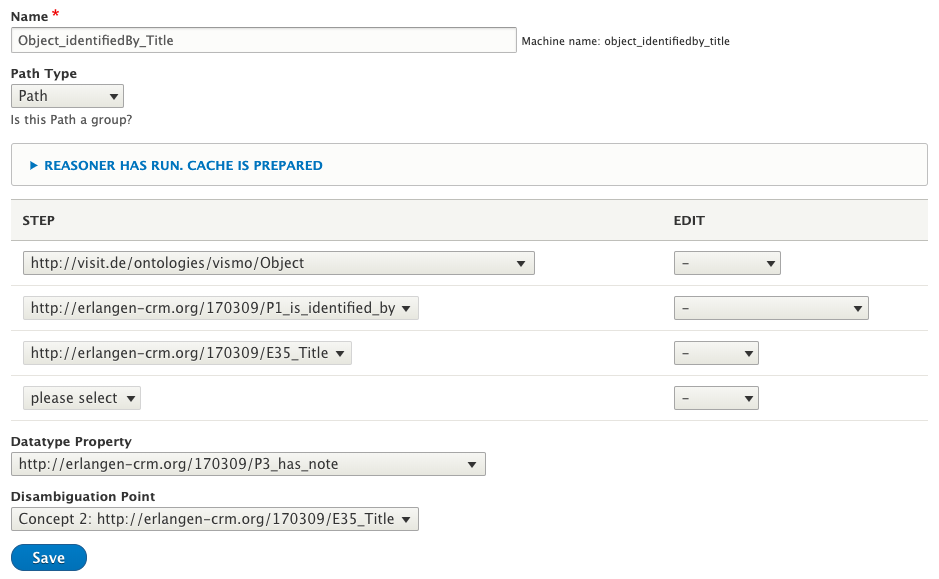
\includegraphics[width=\textwidth]{Figures/berndl/pathsDetails1}
    \caption{\label{fig:pathsDetails1} Erste Maske zum Editieren eines \wisski Pfads.}
\end{figure}

Wird die aktuelle Einstellung des Pfads gespeichert, öffnet sich die zweite Maske zur Konfiguration eines \wisski Pfads. Ausgehend von dem aktuellen Beispiel eines Objekt-Titels ist dies in \autoref{fig:pathsDetails2} zu sehen. Die ersten vier Einstellungen werden automatisch vom System gesetzt, und sollten in der Regel nicht angepasst werden müssen. Wichtig sind die vier unteren Einstellungen, welche den Datentypen des aktuell betrachteten Pfads definieren, indem zuerst der allgemeine Datentyp gesetzt wird und in den folgenden drei Einstellungen lässt sich einstellen, wie dieser Datentyp später in der Eingabemaske des \wisski Systems aussehen soll. In unserem Beispiel kann ein Text in einem einfachen Textfeld angelegt werden. Zusätzlich dazu kann die Kardinalität für das entsprechende Feld festgelegt werden.

\begin{figure}[htb]
    \centering
    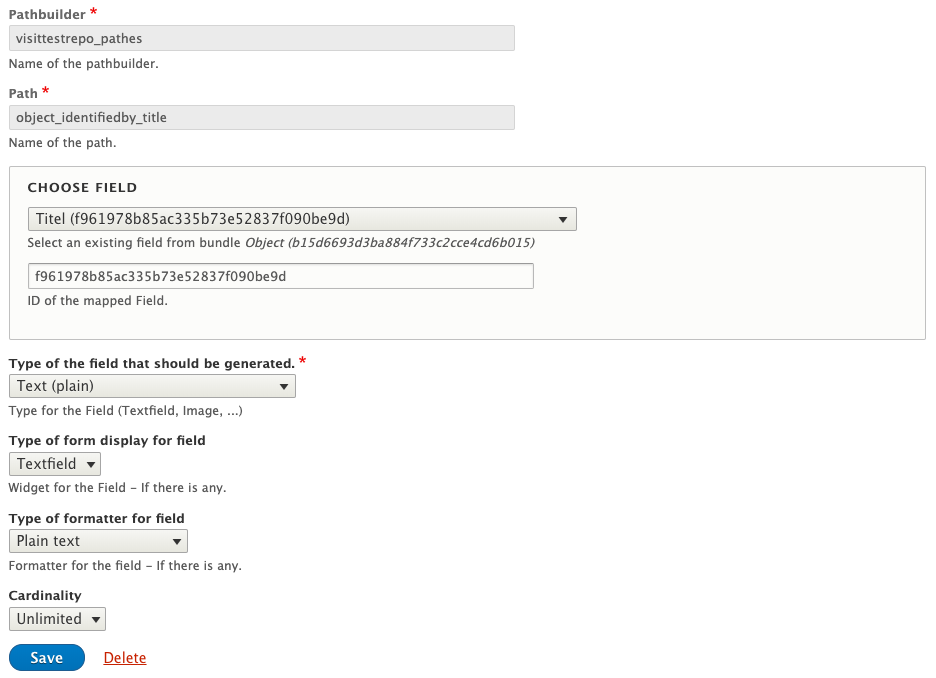
\includegraphics[width=\textwidth]{Figures/berndl/pathsDetails2}
    \caption{\label{fig:pathsDetails2} Zweite Maske zum Editieren eines \wisski Pfads.}
\end{figure}

\autoref{fig:paths2} zeigt weiterhin ein Beispiel für einen Pfad, welcher eine Relation zwischen zwei Datenbankobjekten definiert. In diesem Falle handelt es sich semantisch um eine Beziehung zwischen Teilobjekten, also dass ein Objekt ein Teil eines zweiten Objekts ist. Um dies zu tun ist der Datentyp \texttt{\q{Entity reference}} nötig, und dass der Pfad in der entsprechend zu referenzierenden Klasse endet: wie in diesem Fall \texttt{\q{http://\-visit.\-de/\-ont\-o\-lo\-gies/\-vis\-mo/\-Ob\-ject}}.

\begin{figure}[htb]
    \centering
    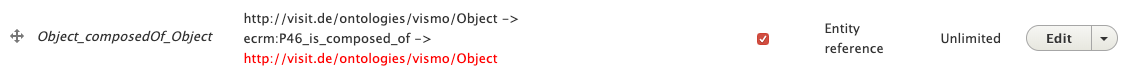
\includegraphics[width=\textwidth]{Figures/berndl/paths2}
    \caption{\label{fig:paths2} Beispiel-Pfad aus der \wisski Konfiguration des \visit Projekts für eine Relation zwischen zwei Entitäten der Datenbank.}
\end{figure}

Zwei weitere wichtige Punkte der \wisski Konfiguration sind in obigen Beispielen zu sehen:

\begin{description}
	\item[Anordnung der Pfade] Die Anordnung der Pfade spielt eine wichtige Rolle in der Konfiguration eines \wisski Systems. Dies ist auf der linken Seite in \autoref{fig:pathbuilder} und der Übersicht der Pfade eines Pathbuilders zu sehen. Die Pfade können dort (durch drag\&drop der \q{Kreuzchen} links neben einer Pfad-ID) in verschiedene Reihenfolgen bzw. Gruppierungen gebracht werden, um somit die Zugehörigkeit eines Pfads zu einer Gruppe, bzw. sogar einer Gruppe zu einer Obergruppe zu definieren. Dies wird getan, indem ein Pfad \q{unter} und dann \q{eine Ebene nach rechts} geschoben wird, wie dies im Beispiel für die ersten beiden Pfade zu sehen ist (ebenfalls in \autoref{fig:paths1} zu sehen). Eine Untergruppe zum Objekt bildet zum Beispiel der Pfad mit der ID \texttt{\q{Object\_Dating}}, welche ihrerseits wieder vier Pfade unter sich zusammen führt. Dies ist wichtig, da das Setzen eines dieser Pfade nicht jeweils einen eigenen Zwischenknoten (mit dem RDF Typen \texttt{\q{http://\-visit.\-de/\-ont\-o\-lo\-gies/\-vis\-mo/\-Da\-ting}}) erzeugen soll, sondern alle vier Pfade den selben Zwischenknoten benutzen sollen.
	\item[Disambiguierung] Die Disambiguierung bezieht sich - seicht formuliert - ähnlich wie die oben beschriebene Anordnung und Untergruppen indirekt auf die korrekte Zuweisung von Knoten zu ihren entsprechenden Objekten. Die Disambiguierung ist in den Pfaden durch die rot geschriebenen Teile zu sehen. Sie weißt das hinterliegende System an, dass alles was ab diesem Punkt im Pfad definiert ist, einzigartig im System gespeichert werden soll. Dadurch können keine Duplikate mit genau der selben Konfiguration entstehen. Dies lässt sich einfach am obigen Beispiel erläutern: die Disambiguierung für den Objekttitel beginnt ab dem \texttt{\q{ecrm:E35\_Title}} Knoten, der weiterhin nur die RDF Eigenschaft \texttt{\q{http://erlangen-crm.org/170309/P3\_has\_note}} besitzt. Durch die Disambiguierung an dieser Stelle wird das System keinen zweiten Knoten erstellen, der den selben Titel in der Notiz-Eigenschaft besitzt. Damit wird sichergestellt, dass zum Beispiel keine zwei Objekte mit dem Titel \q{Mona Lisa} erstellt werden können. Technisch verweist das System im Hintergrund bei verweis auf diesen Knoten somit immer auf genau diesen einen Knoten - wie beschrieben werden \textit{keine} Duplikate davon erstellt. Die Disambiguierung eines Pfads kann in der Maske mit dem Feld \texttt{\q{Disambiguation Point}} vorgenommen werden, die in \autoref{fig:pathsDetails1} zu sehen ist.
\end{description}

Die Informationen und die Konfiguration des Pathbuilders wird vom \wisski System weiterhin genutzt, um Ein- sowie Ausgabeinterfaces für die Hauptobjekte des Pathbuilders zu erzeugen. Über die Create-Seite des \wisski Systems (zu sehen in \autoref{fig:wisskiCreate} im Appendix) ist unter anderem das Eingabe-Interface für die Ausstellungsobjekte (Object) zu erreichen, dieses ist in \autoref{fig:wisskiCreateObject} im Appendix zu sehen. Nachdem Objekte über dieses erstellt wurden, können diese per Navigate- und Find-Seite des \wisski Systems eingesehen werden. Ein Beispiel für das Ausgabeinterface einer Partisane aus dem \visit Projekt ist in \autoref{fig:wisskiViewObject} im Appendix zu sehen.

\subsection{Technischer Zugang zu den Metadaten - die ViSIT REST API}\label{sec:rest}

Das oben beschriebene \wisski System ist entworfen, um im \visit Kontext Zugang für Geisteswissenschaftler, Museumsmitarbeiter und allgemein forschenden Personen zu schaffen. Weiterhin war es im \visit Projekt aber ebenfalls nötig, einen technischen Zugang zu den über \wisski erzeugten Daten zu gewährleisten. Diesen technischen Zugang verwenden weiter verarbeitende Komponenten des Projekts, beschrieben in den Kapiteln 4 bis 8. Ziel ist es ebenfalls, die Informationen der RDF Daten zu vermitteln, ohne dass der Empfänger mit RDF oder anderen semantischen Technologien in Berührung kommen muss.
% TODO insert \autoref{} bis \autoref{}.

Um dies auf standardisierte Weise durchzuführen, ist die Wahl auf eine serverseitige REST API gefallen, die mit den weiteren technischen Komponenten via HTTP kommunizieren kann. Die REST API ist in Java geschrieben und mit dem Spring Framework\footnote{\url{https://spring.io/}} umgesetzt. Die Entwicklung ist in einem Repository im allgemeinen \visit Projekt Bitbucket: \url{https://bitbucket.org/visit2016/metadb-rest-api/}. Eine direkte Kommunikation der aktuell installierten Version der REST API ist stets (sowohl auf dem produktiven Server als auch dem Testsystem) unter der URL Endung \texttt{\q{.../\-me\-ta\-d\-b-rest-api/\-swagger-ui.html}} zu finden.

Dieses Kapitel beschreibt weiterhin die allgemeine Umsetzung der API, dessen Hintergründe, sowie technische Eigenheiten wie Datenmodelle usw. Jedoch sind \textit{die wichtigsten technischen Details zur Verwendung der \visit REST API} in \autoref{sec:features} beschrieben. Dort werden unter anderem wichtige Skripte zur Inbetriebnahme der API erklärt, sowie der Prozess des Deployments erläutert.

Thematisch lässt sich die REST API in folgende Teile aufteilen, die unterschiedliche Aufgabenbereiche übernehmen:

\begin{description}
	\item[Digital Representations:] Die Digital Representations - zu deutsch digitale Repräsentationen - stellen die Verbindungen zwischen Metadaten und zugehörigen Mediendaten dar. Hierzu sind sie ein Eintrag in der Metadatenbank, die zu entsprechenden Entitäten hinzugefügt werden, und dabei verschiedene technische Details zu den Mediendaten beinhaltet. Die REST API bietet hierfür die Möglichkeiten, über HTTP entsprechende Digital Representations zu erzeugen, schreiben, bearbeiten, und zu löschen. Den Repräsentationen liegt folgendes (RDF) Modell, aufgezeigt in \autoref{fig:digrep}, zugrunde:
	
	\begin{figure}[htb]
    	\centering
	    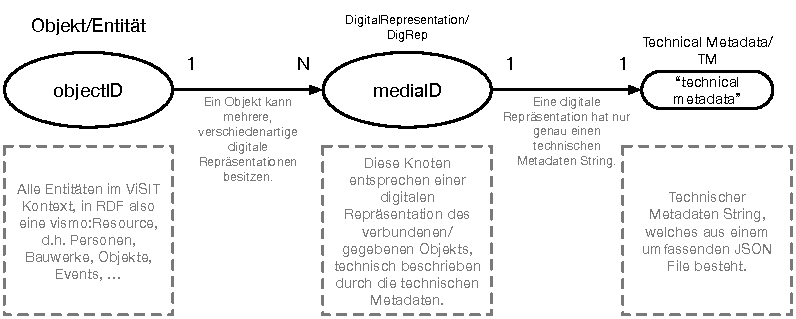
\includegraphics[width=\textwidth]{Figures/berndl/digrep}
    	\caption{\label{fig:digrep} Modell der digitalen Repräsentationen.}
	\end{figure}
	
	Die möglichen API Funktionen sind, in \autoref{tab:digrepapi} die folgenden (die API Pfade sind relativ zur jeweiligen REST API angegeben):
	
	\begin{table}[htb]
		\centering
		\begin{tabular}{|l|l|p{1.5cm}|p{5cm}|}
			\hline
			\texttt{HTTP} & \texttt{API Pfad} & \texttt{Request Params} & \texttt{Kurzbeschreibung} \\
			\hline
			\hline
			GET & /digrep/media & id & Gibt TM String des mit der \q{id} spezifizierten DigRep Knotens zurück. \\
			\hline
			PUT & /digrep/media & id, newData & Updated den TM String durch \q{newData} des per \q{id} spezifizierten DigRep Knotens. \\
			\hline
			DELETE & /digrep/media & id & Löscht den durch die \q{id} spezifizierten DigRep Knoten. \\
			\hline
			GET & /digrep/object & id & Gibt alle TM Strings und deren DigRep Knoten IDs zurück. \\
			\hline
			POST & /digrep/object & id & Legt einen neuen DigRep Knoten für das Objekt mit der gegebenen \q{id} an. \\
			\hline
			DELETE & /digrep/object & mediaId, objectId & Löscht den DigRep Knoten mit der ID \q{mediaID}, zugehörig zum Objekt mit der ID \q{objectID}. \\
			\hline
		\end{tabular}
		\caption{API Funktionen für die Digital Representations.}
		\label{tab:digrepapi}
	\end{table}

	\item[Objekte:] Dieser Bereich der API dient hauptsächlich zum Auslesen der Datenbankobjekte bzw. Entitäten, die über \wisski in der Metadatenbank angelegt wurden. Diese API Schnittstelle erfüllt die Anforderung, die bereits am Anfang dieses Unterkapitels beschrieben wurde: die Gewährleistung des technischen Auslesens der Metadaten in einem \textit{nicht}-Semantic Web Format, in diesem Falle JSON. Dieses JSON beinhaltet alle Informationen, die entsprechend als RDF Metadaten auf der Datenbank vorhanden sind. \autoref{lst:json} im Appendix gibt eine Art Schema für diesen Output an. Dort werden alle möglichen Felder mit ID, Datentyp und den potenziell referenzierten Typen einer Referenz angegeben. Zum Auslesen der Objekte bietet die API zwei mögliche API Funktionen aus \autoref{tab:objectapi}:
	
	\begin{table}[htb]
		\centering
		\begin{tabular}{|l|l|p{2cm}|p{5cm}|}
			\hline
			\texttt{HTTP} & \texttt{API Pfad} & \texttt{Request Params} & \texttt{Kurzbeschreibung} \\
			\hline
			\hline
			GET & /object & id & Gibt die JSON Repräsentation des Objekts mit der ID \q{id} zurück. \\
			\hline
			GET & /wisskiobject & wisskipath & Gibt die JSON Repräsentation des Objekts zurück, welches dem \wisski View Path \q{wisskipath} entspricht. \\
			\hline
		\end{tabular}
		\caption{API Funktionen zum Auslesen von Objekten.}
		\label{tab:objectapi}
	\end{table}
	
	Wichtig zu wissen beim Auslesen der Objekte ist, dass die angesprochene ID der API die RDF ID des Knotens der entsprechenden Entität ist (z.B. \texttt{\q{http://visit.de/data/5c4ae02a2d569}}), während der sogenannte \q{\wisski View Path} derjenige URL Pfad ist, der angezeigt wird, wenn eine Entität per \wisski Oberfläche betrachtet wird (z.B. \texttt{\q{https://\-da\-ta\-base.\-vi\-sit.\-u\-ni-pas\-sau.\-de/\-dru\-pal/\-wis\-ski/\-na\-vi\-gate/\-405/\-view}}).
	
	Weiterhin bietet dieser Bereich der API noch ein zusätzliches Quality of Life Feature: das Zurückgeben der Anzahl an vorhandenen Digital Representations und damit vorhandenen Mediendaten, bezogen auf ein Objekt. Dieses Objekt kann der API, wie beim Auslesen, per RDF ID oder per \wisski View Pfad übergeben werden.
	
	\item[(Upload und Download für Excel:)] TODO add?
\end{description}

Für die REST API ist eine Verschlüsselung umgesetzt, die dem Konzept der \q{basic authentication}\footnote{Erklärt z.B. auf \url{https://swagger.io/docs/specification/authentication/basic-authentication/}} folgt. Mit dieser werden die sogenannten \q{unsicheren} Operationen der API, also diejenigen, die Daten verändern, erzeugen, und löschen dürfen, von unzulässigem Zugriff geschützt. Diese sind im \visit Kontext diejenigen Operationen, die sich auf die DigitalRepresentations beziehen. Alle rein lesenden Zugriffe auf die Metadatenbank sind gemäß dem Linked Open Data Gedanken offen nach aussen.

Für die gesicherten Zugänge der API sind auf dem \visit Server verschiedene \q{User} samt Passwort angelegt, welche auf die jeweils verarbeitenden Applikationen gemünzt werden, dementsprechend die Tablet und Fernrohr Apps, sowie die Kompressions-Komponente. Diese Liste an Usern und Passwort sind am entsprechenden Server im eigenen Bereich des \q{visit} Accounts zu finden und nur für entsprechende Administratoren zugänglich. Die Datei hat den Namen \texttt{\q{users.csv}} und muss \textbf{vor dem Start bzw. dem Deployment} der REST API vorhanden sein, damit diese darauf Zugriff hat.

\subsection{Wichtige Technische Charakteristika der Entwicklung und den Betrieb der Semantischen Datenbank}\label{sec:features}

In diesem Unterabschnitt werden wichtige technische Details zum Betrieb der \visit REST API erläutert. Diese sind wichtig für die Nutzung der API.

\paragraph{Python Script zum Generieren der SPARQL Query Templates}

\textbf{WICHTIG:} Das im Folgenden beschriebene Script muss \textbf{vor} Deployment der REST API ausgeführt werden.

Für den Betrieb der REST API, vor allem zum Auslesen der unterliegenden Metadaten, sind sogenannte SPARQL Query Templates von Nöten. Diese können als Vorlagen für die Abfrage aus der Metadatenbank verstanden werden. Diese Query Templates werden automatisch aufbauend auf dem in \wisski definierten Paths erstellt. So kann, wenn sich die \wisski Pfad Konfiguration ändert, das Script erneut angestoßen werden, um auf die Veränderung zu reagieren und damit die neu hinzugefügten Pfade mit in die Anfragen aufgenommen werden. Dieser Prozess ist in einem Phyton Script gekapselt, welches auf dem \visit Server ausgeführt werden kann.

Wichtigste Information die das Script benötigt sind die Pfad Konfigurationen des \wisski Systems. Diese können als Datei direkt im \wisski System, im Pathbuilder downgeloadet werden. \autoref{fig:download} zeigt diese Funktionalität mit dem \texttt{\q{Create Exportfile}} Button.

	\begin{figure}[htb]
    	\centering
	    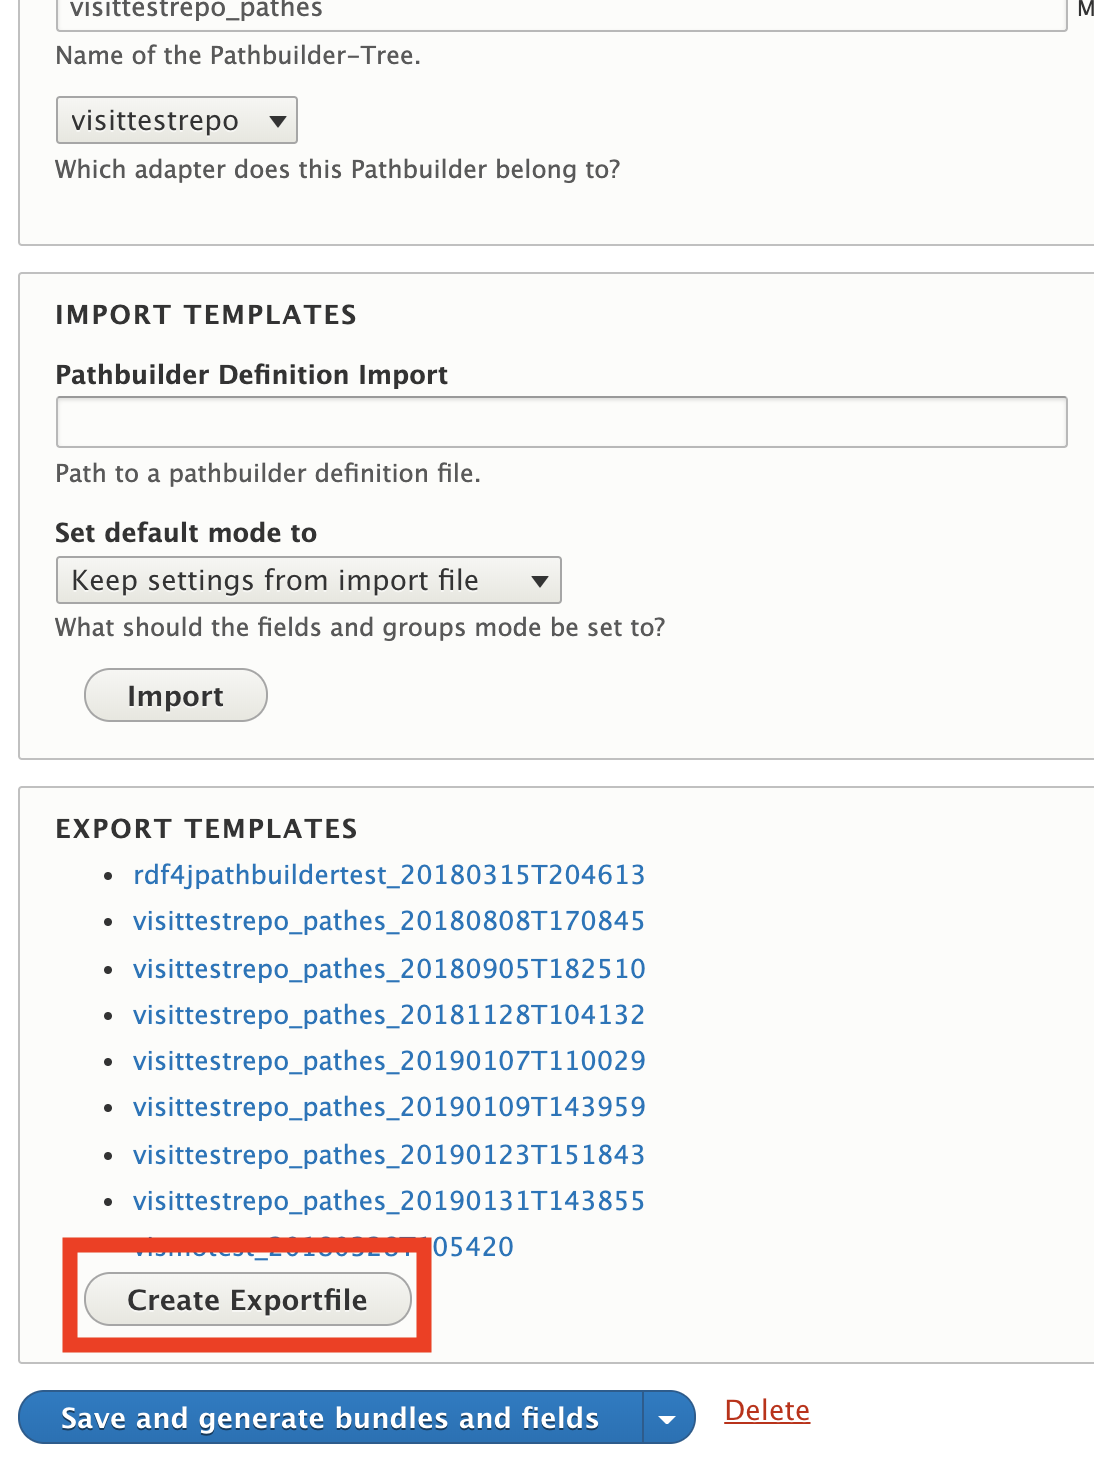
\includegraphics[width=\textwidth]{Figures/berndl/wisskiPathDownload}
    	\caption{\label{fig:download} \wisski Pathbuilder Ansicht, die den Download der Pfad-Datei anbietet.}
	\end{figure}
	
Nach Betätigen des Buttons wird eine aktuelle Datei in die darüber stehende Liste aufgenommen. Durch Drücken dieser kann die Datei anschließend gespeichert werden.

Das Python Script befindet sich auf dem Server im Account \texttt{\q{visit}} im Ordner \texttt{\q{python}} und heißt \texttt{\q{CreateSPARQLTemplatesFromPathsXML.py}}. \textbf{Die Pfad-Datei muss umbenannt werden zu \texttt{\q{paths.xml}} und muss sich im selben Ordner befinden}. Das Ausführen des Scripts kann mit folgendem Befehl ausgeführt werden:

\begin{lstlisting}[style=MyBashStyle, caption={Befehl zum Starten des Python Script zum Erstellen der Query Templates der \visit Metadatenbank.}]
sudo python3 CreateSPARQLTemplatesFromPathsXML.py
\end{lstlisting}

Die Ergebnisse des Scripts werden automatisch in den Ordner \texttt{\q{Templates}} im Hauptordner des Accounts \texttt{\q{visit}} gespeichert, und automatisiert von der REST API benutzt.

\paragraph{Einstellungen zum Deployment der REST API}

Wie oben bereits beschrieben, ist die REST API in einem Repository\footnote{\url{https://bitbucket.org/visit2016/metadb-rest-api/src/master/}} des \visit Haupt-Repositories angelegt.

In der Regel ist das entsprechende Projekt in einem \q{offline Teststatus} bezüglich seiner Konfiguration. Dies bedeutet, dass lokale Tests ausgeführt werden können, um die Funktionen der API lokal zu überprüfen. Sollte die REST API produktiv auf einem Server deployed werden, müssen folgende Änderungen in der Konfiguration durchgeführt werden:

\begin{itemize}
	\item Einbinden der springframework Dependency: In der \texttt{\q{pom.xml}} Maven Konfigurationsdatei des Projekts muss die Dependency für das Artefakt \texttt{\q{spring-boot-starter-tomcat}} auf den scope \texttt{\q{provided}} gesetzt werden. Die entsprechende Einstellung ist in \autoref{fig:springdependency} zu sehen. Wichtig ist, dass Zeile 4 \textbf{nicht} kommentiert ist.
	
	\begin{figure}[htb]
    	\centering
	    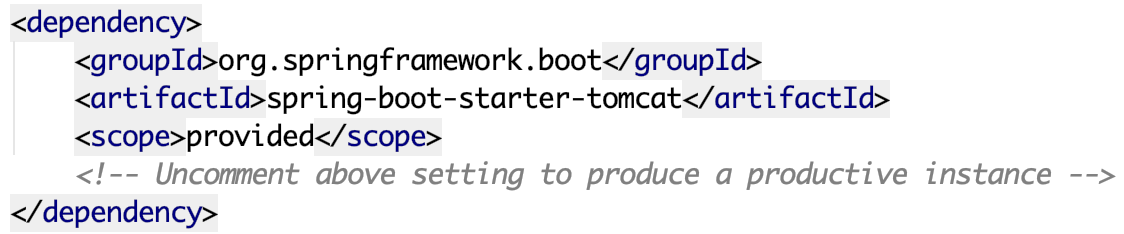
\includegraphics[width=\textwidth]{Figures/berndl/springDependency}
    	\caption{\label{fig:springdependency} pom.xml Konfiguration zum produktiven Deployment der REST API.}
	\end{figure}
	
	\item Verbindung zum entsprechenden Triplestore: Weiterhin ist es nötig, die REST API mit dem Triplestore zu verbinden, mit dem das aktuell verwendete System, im speziellen das \wisski System, arbeitet. Diese Verbindung wird in der REST API in der Konfigurationsdatei \texttt{\q{application.properties}} gesetzt. Dabei muss der query und der update Endpunkt URLs des jeweiligen Triplestores angegeben werden. Im offline Modus sind die beiden URLs auf \texttt{\q{none}} gesetzt, während sie für den Produktiv-Modus der API auf den entsprechenden Triplestore eingestellt werden müssen. In \autoref{fig:triplestoreconfig} ist die Konfiguration für den offline Modus zu sehen, während ebenfalls zwei vordefinierte URL Pärchen zu sehen sind, welche für den \visit Test- und Produktiv-Server stehen.
	
	\begin{figure}[htb]
    	\centering
	    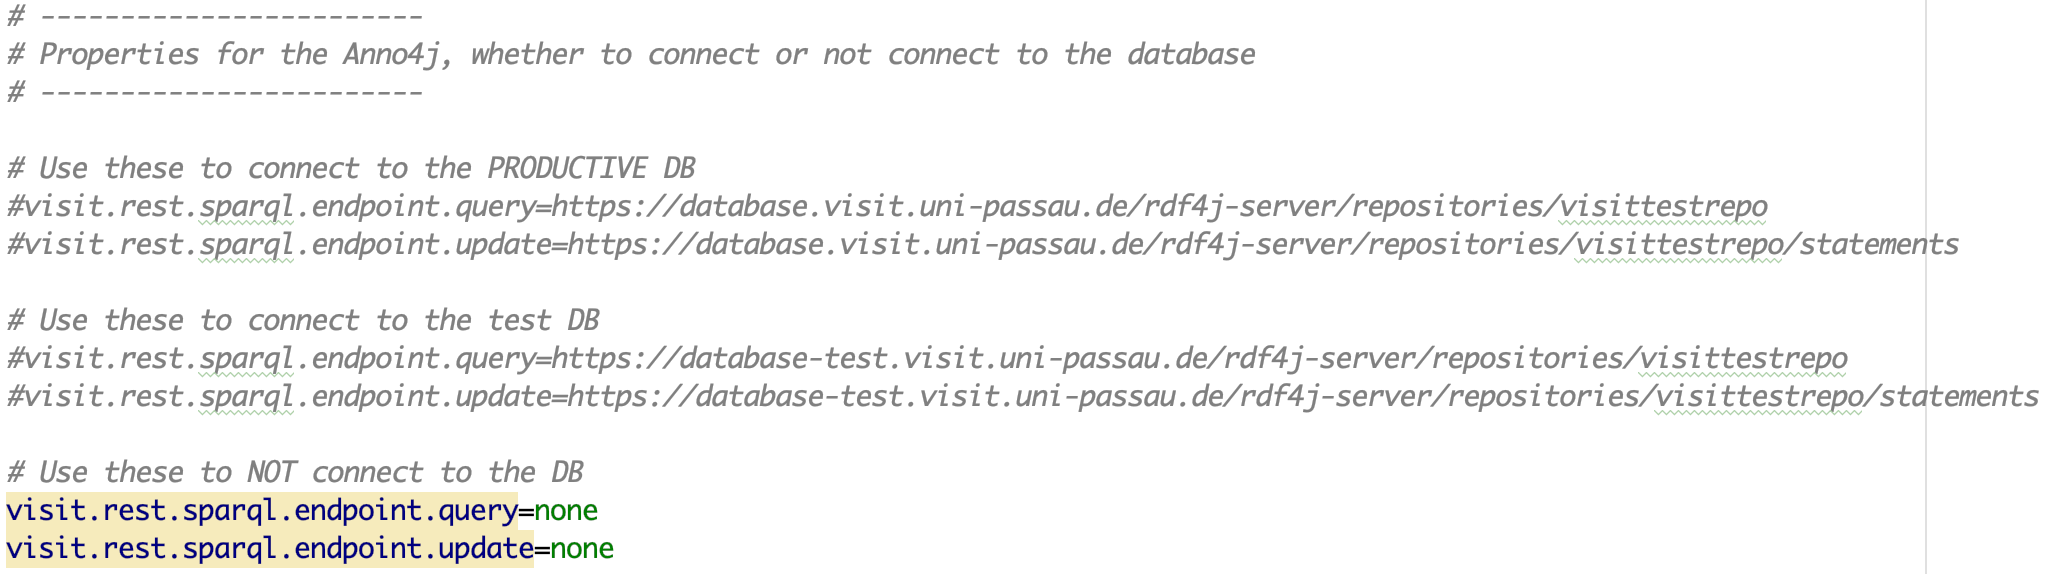
\includegraphics[width=\textwidth]{Figures/berndl/triplestoreConfig}
    	\caption{\label{fig:triplestoreconfig} Einstellungen zum Verbinden des Triplestores. Hier gezeigt: lokale Konfiguration, während die Konfiguration für Produktiv- und Testsystem oben vorhanden aber auskommentiert ist.}
	\end{figure}
\end{itemize}

\subsection{Zusatzfeatures - Erweiterung der Bedienbarkeit der Semantischen Datenbank}\label{sec:additional_features}

copy and paste feature

excel importer

\subsection{Semantische Datenbank - FAQ und häufig auftretende Probleme}\label{sec:faqSW}

Nachdem bis jetzt alle Details bezüglich der Metadatenbank und dessen Umgang erläutert wurden, führt dieses Unterkapitel eine Zusammenfassung von bekannten \q{Problemen} in Kombination mit Lösungen an, die im produktiven Betrieb der Datenbank entstehen können. Bei Auftreten eines dieser Probleme sollte die Datenbank durch Einsatz der aufgeführten Lösung wieder in einen funktionierenden Zustand überführt werden können.

\paragraph{WissKI Cache Flush}

Bei manchen Konfigurations-Änderungen kann es passieren, dass diese erst \q{online} geschaltet werden, wenn der Cache des Drupal Systems geleert wird. Dies ist zum Beispiel der Fall, wenn ein Thumbnail für ein Objekt in der Metadatenbank hochgeladen wird. Der produktive Server ist so konfiguriert, dass einmal am Tag ein solcher Cache Flush durchgeführt wird. Sollten die jeweiligen Informationen durch die Konfiguration jedoch sofort benötigt werden, kann ein Cache Flush auch per Hand am Server ausgeführt werden. Dazu muss in das Verzeichnis der Drupal Installation gewechselt werden (\texttt{/var/www/html/drupal}) und folgender Befehl ausgeführt werden:

\begin{lstlisting}[style=MyBashStyle, caption={Befehl für einen Cache Flush eines Drupal Systems.}]
drush cr 
\end{lstlisting}

\paragraph{Recompute Hierarchy in WissKI}

Wenn die dem WissKI System unterliegende Ontologie ausgetauscht oder upgedated wird, kann es sein, dass das System über diese Ontologie eine neue Hierarchie generieren muss. Das neue Berechnen der Ontologie kann in der Übersicht des SALZ Adapters (siehe \autoref{sec:wisski}, Funktionalität ganz unten aufklappbar) angestoßen werden.

\paragraph{Updates von Drupal, Maintenance Mode}

Von Zeit zu Zeit wird eine neue Version von Drupal released. Dies ist für die Metadatenbank theoretisch irrelevant, wenn es nur ein Minor Update ist (diese sollten aber im Bezug auf aktuelle Software trotzdem eingespielt werden). Ein Major Update führt in der Regel jedoch dazu, dass das Drupal System in den Maintenance Mode versetzt wird - ein Status in dem das System aus Sicherheitsgründen offline geschaltet wird. Deswegen ist hier ein Update durchzuführen.

Updates des Drupal Systems können (in seltenen Fällen) entweder im Drupal Interface selbst durchgeführt werden (Reiter \q{Extend}, dann auf Link für \q{available updates} drücken). In der Regel führt man die Updates (auch von anderen Modulen) direkt am Server durch. Dafür in das Verzeichnis der Drupal Installation wechseln (\texttt{/var/www/html/drupal}) und folgenden Befehl ausführen:

\begin{lstlisting}[style=MyBashStyle, caption={Befehl zum Updaten einer Drupal Installation.}]
sudo composer update --with-all-dependencies 
\end{lstlisting}

Möglicherweise müssen im Konflikt stehende Abhängigkeiten von Hand gelöst werden. Dazu Schritt für Schritt die einzelnen Dependencies updaten und am Ende nochmals obigen Befehl ausführen.

\paragraph{RDF4J Workbench Access}

Um direkt auf dem unterliegenden Triplestore zu arbeiten, kann auf die RDF4J Workbench zugegriffen werden (URL: \texttt{\url{https://database.visit.uni-passau.de/rdf4j-workbench}}. In manchen Fällen leitet das Aufrufen der Homepage zu einem Prompt, der nach der URL, sowie Benutzer und Passwort verlangt. Für den Server ist kein User angelegt, deswegen können die beiden Felder für Benutzer und Passwort leer gelassen werden. Jedoch ist manchmal die angegebene URL inkorrekt, da \texttt{\q{http}} anstatt \texttt{\q{https}} in der URL steht. Dieses muss angepasst werden, dann kann auf den Triplestore zugegriffen werden.

\paragraph{Maven Abhängigkeiten im REST API Projekt}

Im Java Projekt für die ViSIT REST API passiert ab und an der Fall, dass die Abhängigkeiten des Projekts nicht richtig interpretiert werden, was dazu führt, dass einige Packages in den implementierten Klassen als \q{nicht vorhanden} angezeigt werden. Durch ein erneutes Downloaden der Abhängigkeiten (durch das Kommando \texttt{\q{Reimport}} oder falls dies nicht hilft \texttt{\q{Update Maven Indices}} in der obersten \texttt{pom.xml} des Projekts) sollte sich dieses Problem lösen lassen.